\section{\texorpdfstring{Charged-Pion Asymmetries and Comparison with Previous Analyses}{Comparison with Previous Analyses}}
\label{sec:comparewpreviouse}

The comparison of $\pi^0$ and $\pi^{\pm}$ asymmetries is of interest because charged pions and $\pi^0$ have similar favored and disfavored Collins fragmentation functions. 
In addition, there are measurements of $A^{UL}_{12}$ and $A^{UC}_{12}$ [cf.~Eqs.~\eqref{eqn:FF7}] by BaBar~\cite{BabarCharged} and Belle~\cite{ChargedPionResult2,ChargedPionResult}. 
Compared to the $\pi^0$ and $\eta$ asymmetries, the charged-pion asymmetries $A^{UL}_{12}$ and $A^{UC}_{12}$ access different combinations of favored and disfavored fragmentation functions as shown in Eqs.~\eqref{eqn:allratiosexpress2}-\eqref{eqn:allratiosexpress3}. In this analysis, the charged--pions-to-thrust opening angle is limited to below 0.3---the same as the $\pi^0$ opening angle constraint---to facilitate the comparison.

%The $A^{UL}_{12}$ and $A^{UC}_{12}$ double ratios for charged pions are given by: %in Eq.~\eqref{eqn:chargeddoubleratio1},.~\eqref{eqn:chargeddoubleratio2}. 
%
%\begin{equation}
%\begin{aligned}
%A^{UL|}_{12}&=&\frac{A^U_{12}}{A^L_{12}}&=&\frac{\pi^+\pi^-}{\pi^+\pi^++\pi^-\pi^-}
%\label{eqn:chargeddoubleratio1}
%\end{aligned}
%\end{equation}
%and
%\begin{equation}
%\begin{aligned}
%A^{UC|}_{12}&=&\frac{A^U}{A^C}&=&\frac{\pi^+\pi^-}{\pi^+\pi^++\pi^-\pi^-+\pi^+\pi^-+\pi^-\pi^+}.
%\label{eqn:chargeddoubleratio2}
%\end{aligned}
%\end{equation}


The asymmetry $A_{12}^{\pi^0}$ can be expressed in terms of fragmentation functions as shown in Eq.~(\ref{eqn:FF5}). %\cite{BabarCharged}\cite{ChargedPionResult2}
The charged-pion double ratios $R^{UL}_{12}$ and $R^{UC}_{12}$ can be written in terms of the various fragmentation functions as
%
\begin{equation}
\begin{aligned}
R^{UL}_{12}&=1+\cos(\phi_1+\phi_2)\frac{\sin^2(\theta)}{1+\cos^2(\theta)}\\
&\times\bigg\{\frac{5(H^{\bot,fav}_1H^{\bot,fav}_1+H^{\bot,dis}_1H^{\bot,dis}_1)+2H^{\bot,dis}_{1,s\rightarrow\pi}H^{\bot,dis}_{1,s\rightarrow\pi}}{5(D^{fav}_1D^{fav}_1+D^{dis}_1 D^{dis}_1)+2D^{dis}_{1,s\rightarrow\pi}D^{dis}_{1,s\rightarrow\pi}}\\
&-\frac{5H^{\bot,fav}_1 H^{\bot,dis}_1+H^{\bot,dis}_{1,s\rightarrow\pi}H^{\bot,dis}_{1,s\rightarrow\pi}}{5D^{fav}_1D^{dis}_1 +D^{dis}_{1,s\rightarrow\pi}D^{dis}_{1,s\rightarrow\pi}} \bigg\} 
\end{aligned}
\label{eqn:allratiosexpress2}
\end{equation}
\begin{equation}
\begin{aligned}
R^{UC}_{12}&=1+\cos(\phi_1+\phi_2)\frac{\sin^2(\theta)}{1+\cos^2(\theta)}\\
&\times\bigg\{\frac{5(H^{\bot,fav}_1H^{\bot,fav}_1+H^{\bot,dis}_1H^{\bot,dis}_1)+2H^{\bot,dis}_{1,s\rightarrow\pi}H^{\bot,dis}_{1,s\rightarrow\pi}}{5(D^{fav}_1D^{fav}_1+D^{dis}_1D^{dis}_1)+2D^{dis}_{1,s\rightarrow\pi}D^{dis}_{1,s\rightarrow\pi}}\\
&-\frac{5(H^{\bot,fav}_1+H^{\bot,dis}_1)(H^{\bot,dis}_1+H^{\bot,fav}_1)+4H^{\bot,dis}_{1,s\rightarrow\pi}H^{\bot,dis}_{1,s\rightarrow\pi}}{5(D^{fav}_1+D^{dis}_1)(D^{dis}_1+D^{fav}_1)+4D^{dis}_{1,s\rightarrow\pi}D^{dis}_{1,s\rightarrow\pi}} \bigg\}
\end{aligned}
\label{eqn:allratiosexpress3}
\end{equation}

Just like for the $\pi^0$ asymmetries, the thrust smearing has to be considered for charged pions. The same method (as described in Section~\ref{sec:pi0thrustcorrection}) is employed here. 
%The statistics are too low to have a reliable thrust correction factor for some bins, and those numbers are estimated based on the Belle Monte Carlo results. 
%Details about these estimations can be found in section~\ref{sec:appendix}. 
%For this comparison, we only apply the  thrust correction to the charged pion asymmetries. 
\iffalse
\begin{figure}[H]
  \centering     
  \subfigure[$z_1$ bins]{\label{fig:sinzCN}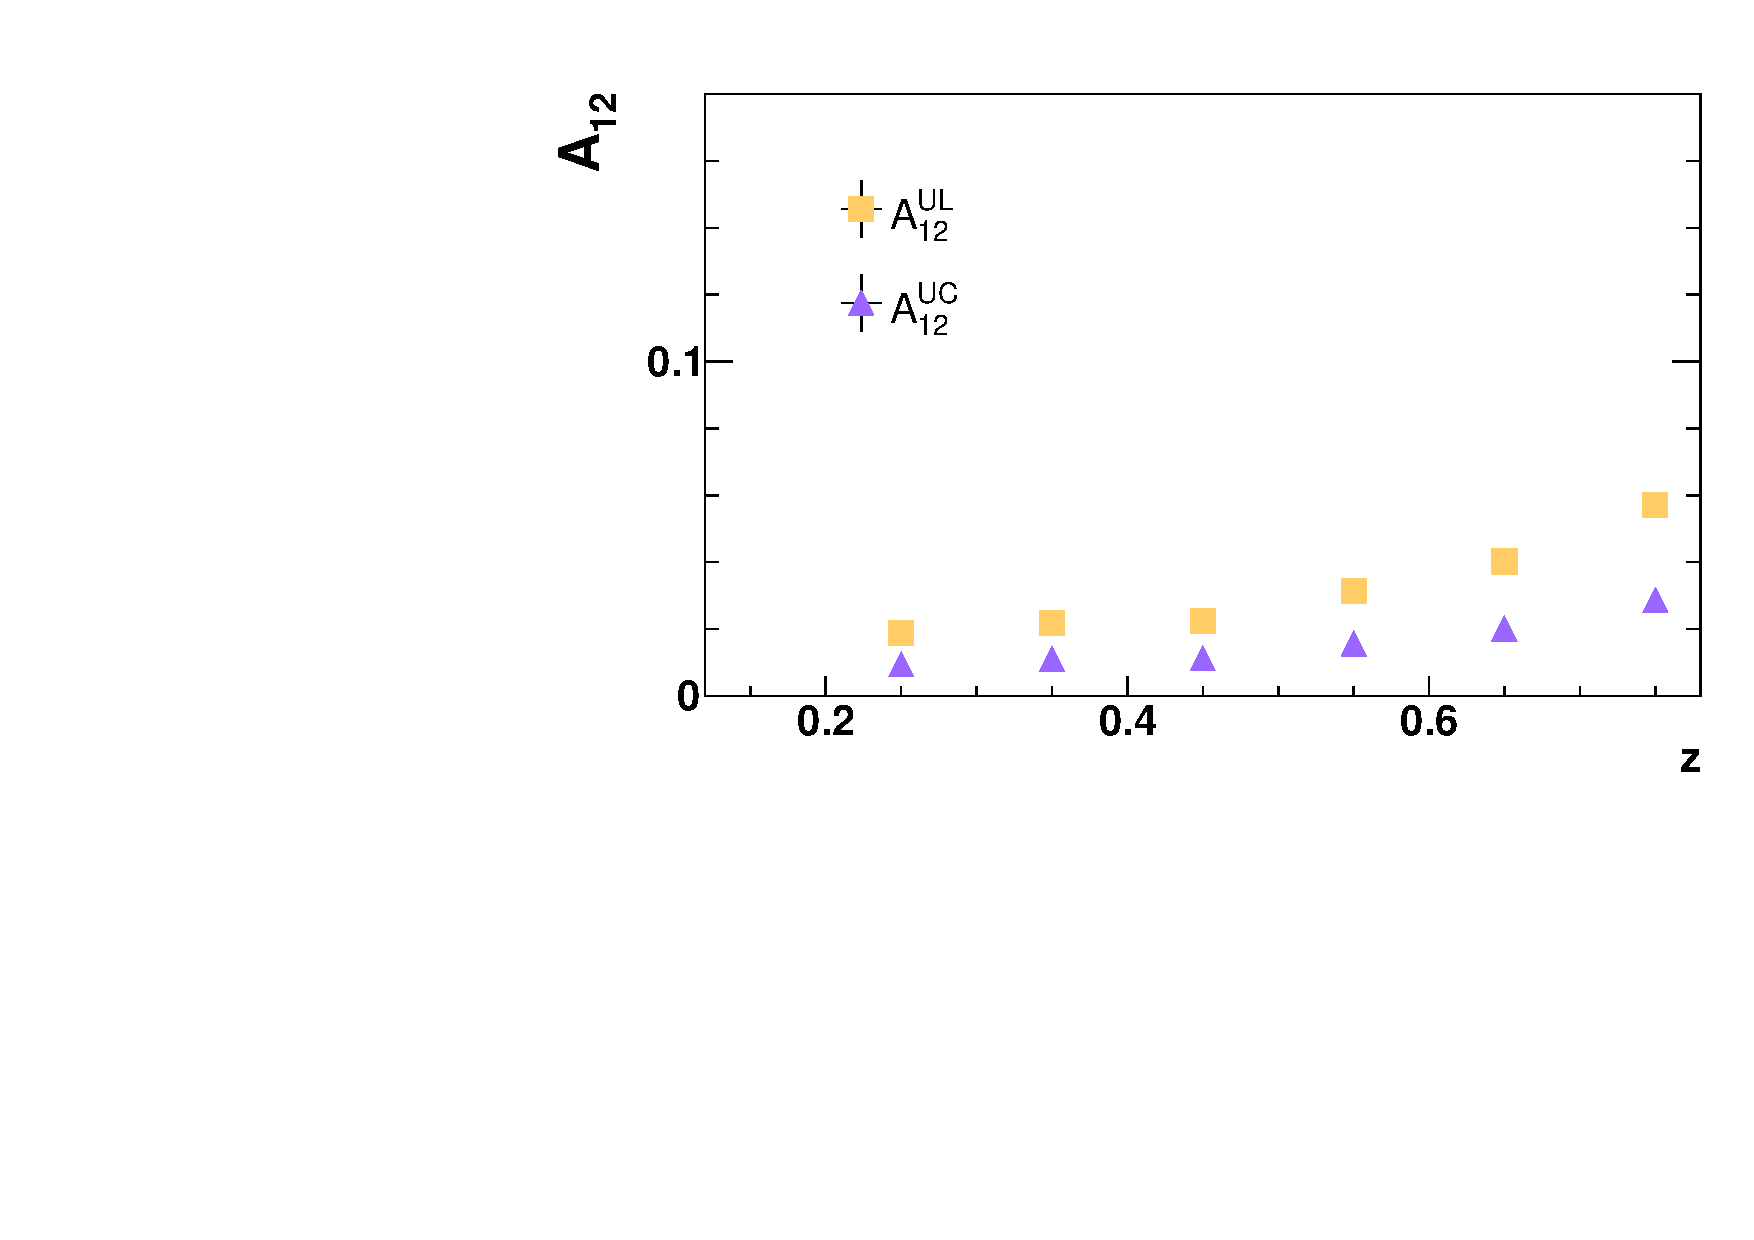
\includegraphics[width=60mm,natwidth=600,natheight=400]{figure_asy/Charged0.pdf}}
  \subfigure[$P_{t1}$ bins]{\label{fig:sinptCN}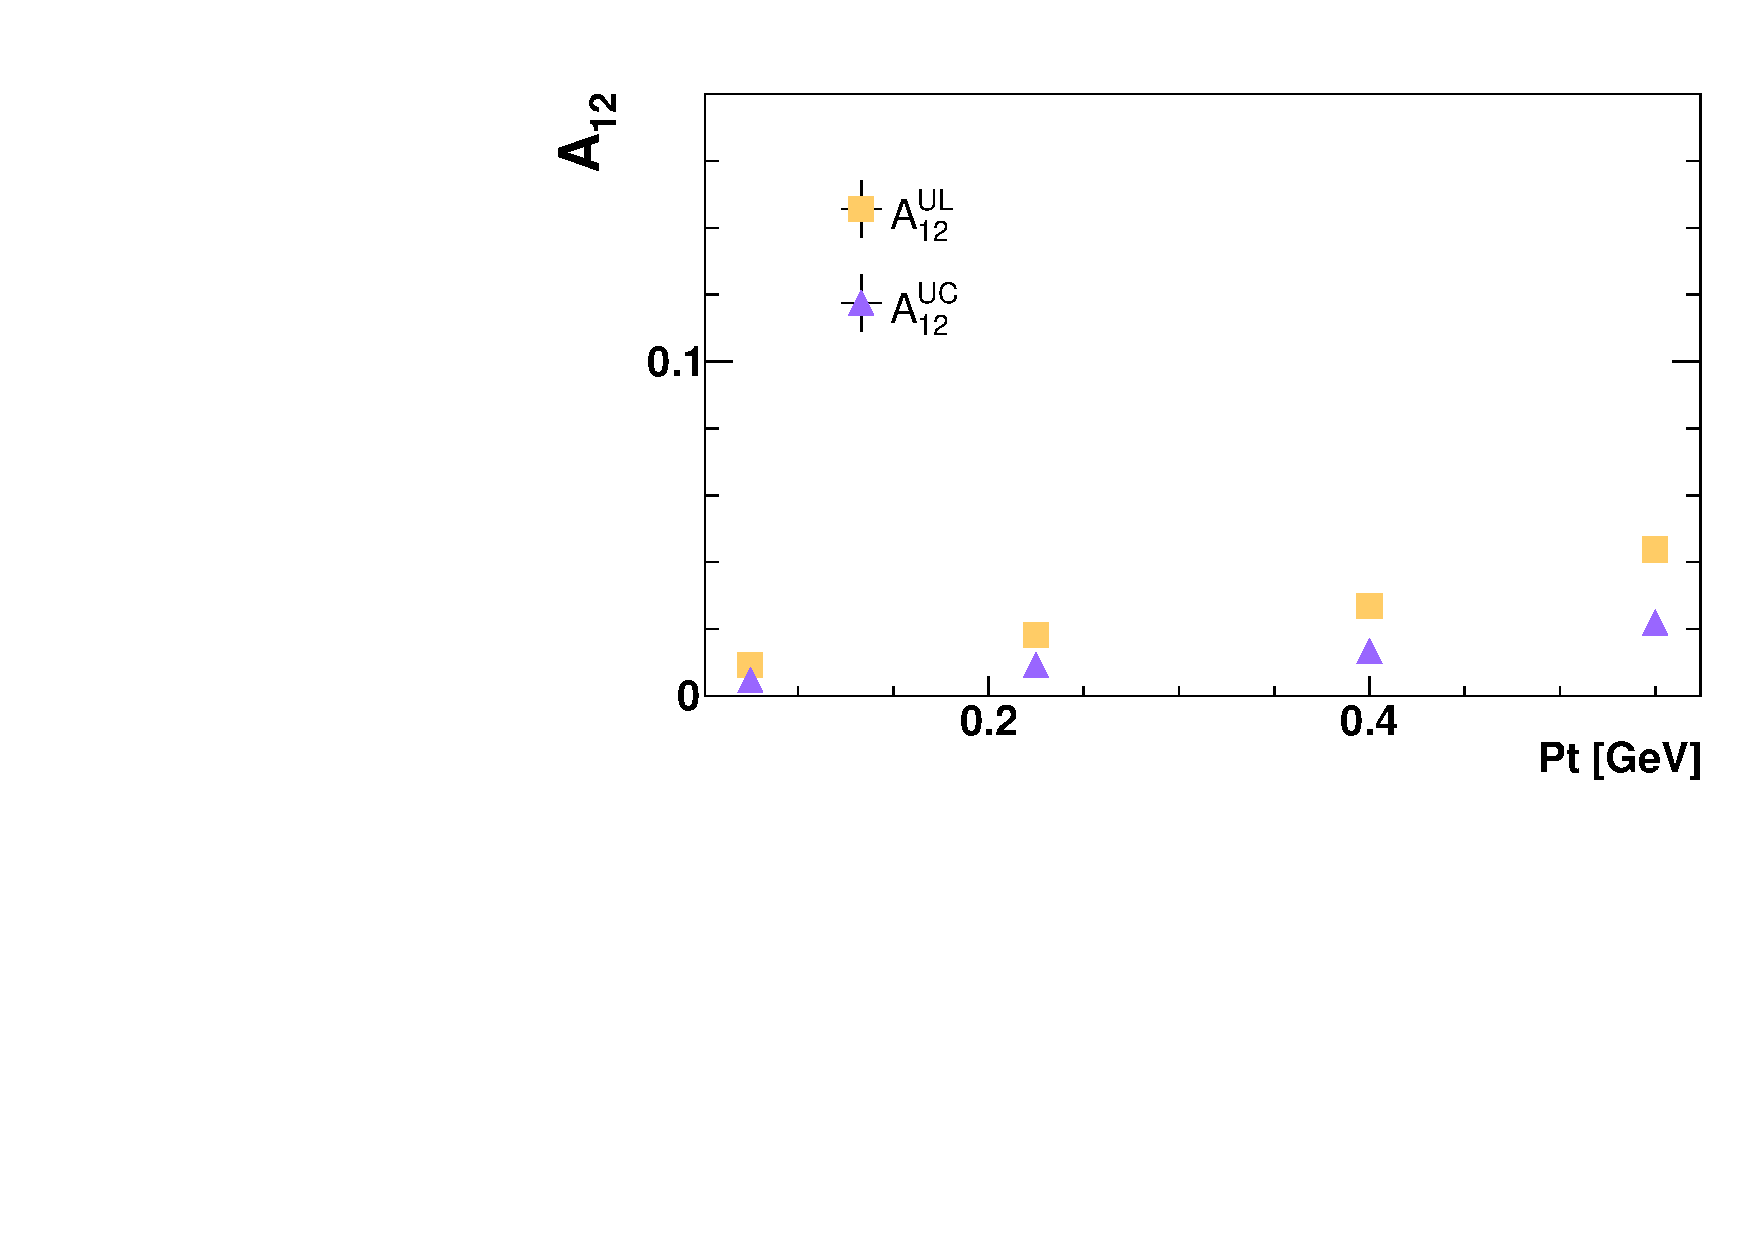
\includegraphics[width=60mm,natwidth=600,natheight=400]{figure_asy/Charged2.pdf}}
  \subfigure[$(z_1,z_2)$ bins]{\label{fig:comzCN}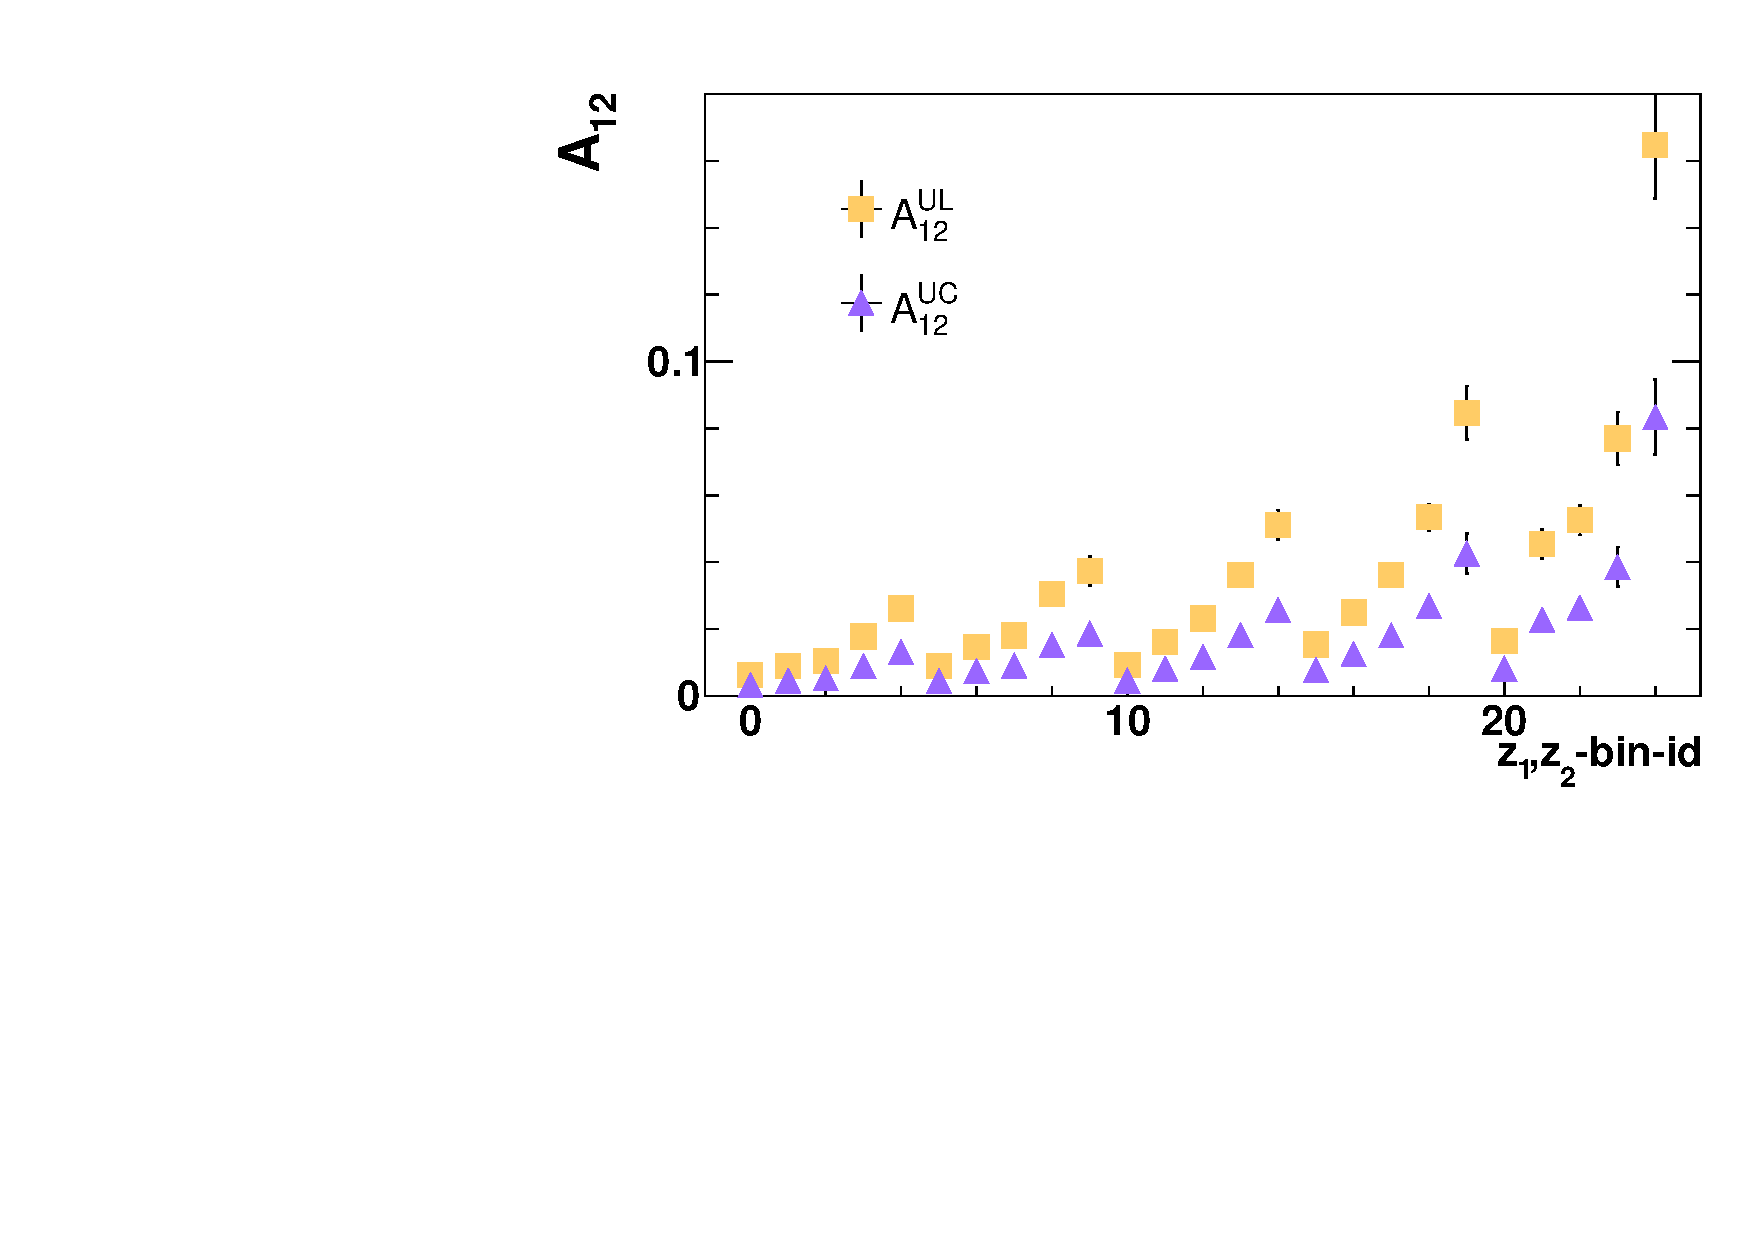
\includegraphics[width=60mm,natwidth=600,natheight=400]{figure_asy/Charged1.pdf}}
  \subfigure[$(P_{t1},P_{t2})$ bins]{\label{fig:comptCN}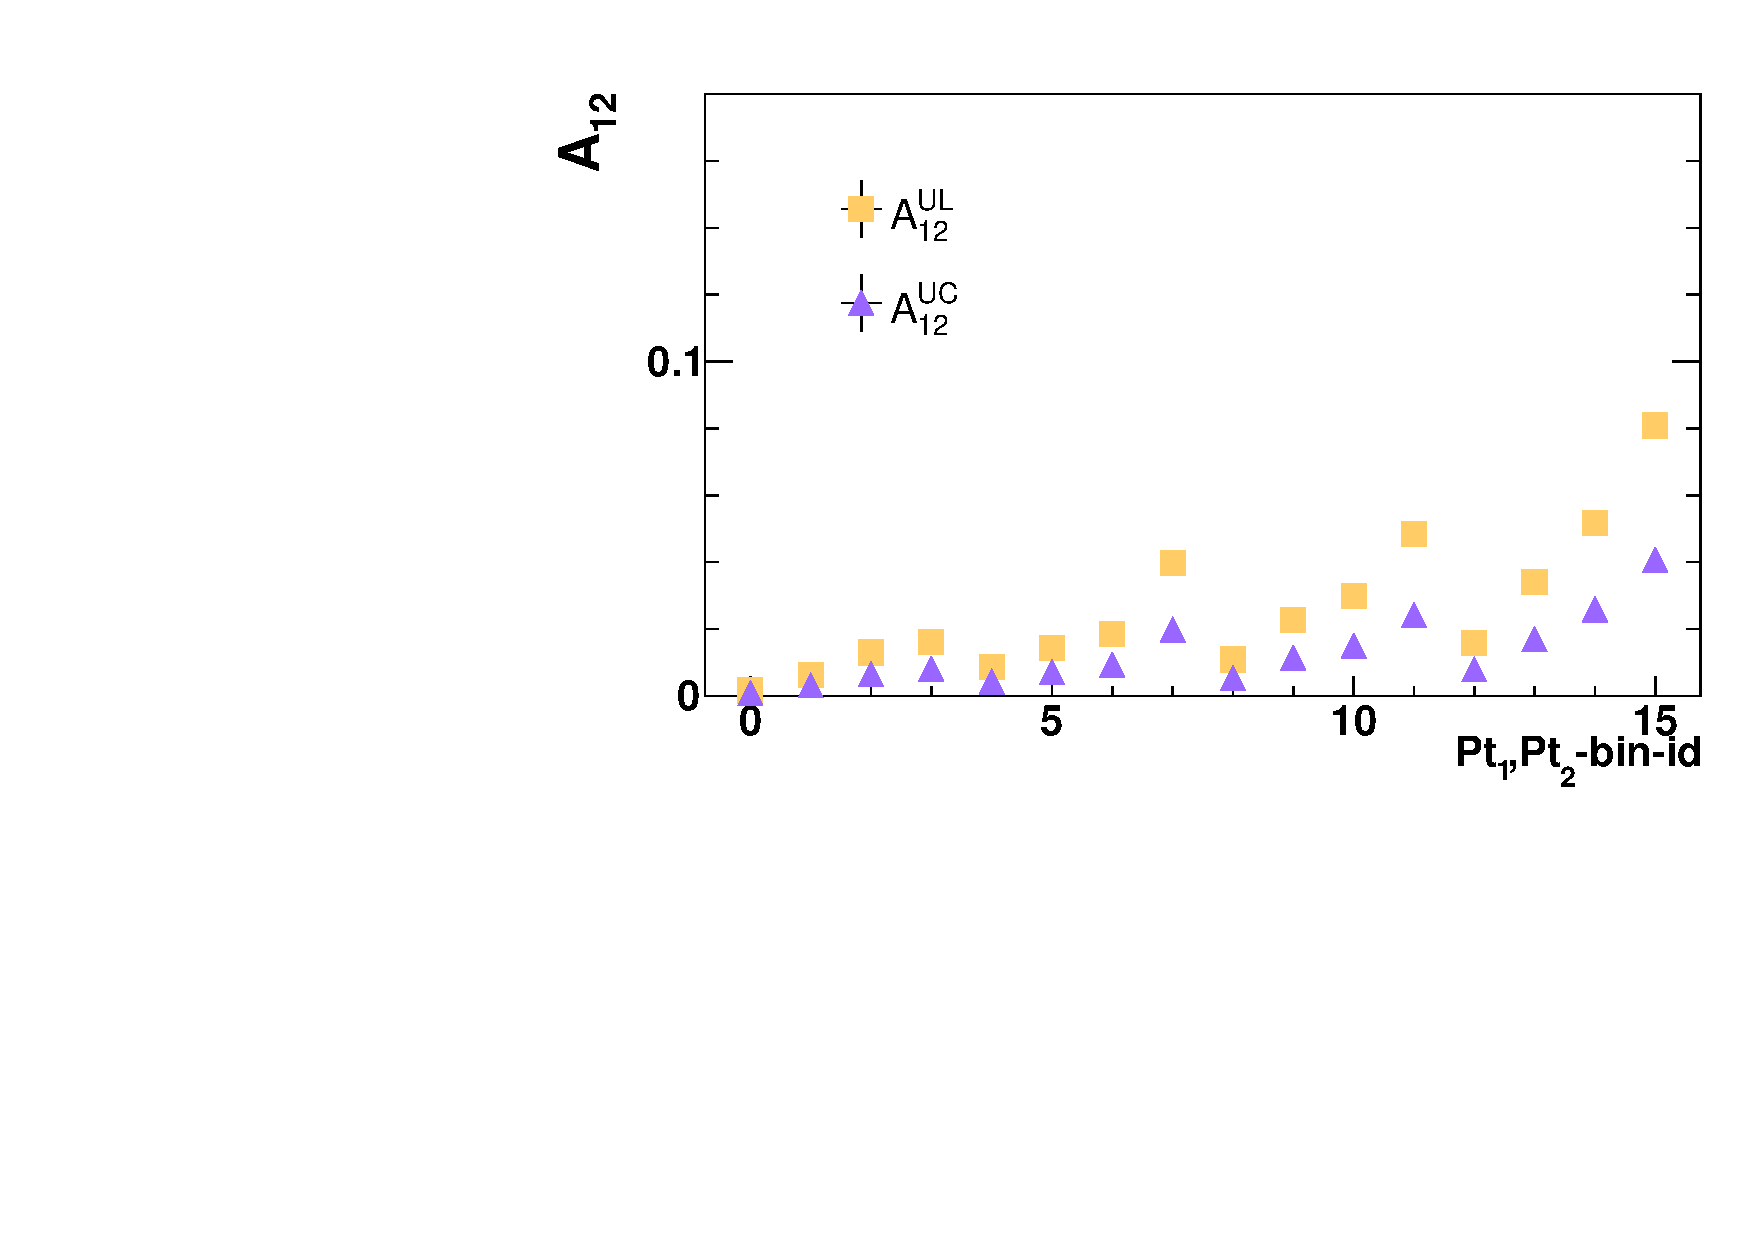
\includegraphics[width=60mm,natwidth=600,natheight=400]{figure_asy/Charged3.pdf}}
  \caption{Charged pion double ratios result for different kinematic bins. The green squares represent no correction result while the purple points are results with thrust smearing correction.}
\label{fig:chargedpion}
\end{figure}
\fi
Figure~\ref{fig:belleCompCharmCorr} shows the comparison with the previous Belle analysis. The agreement is in general good. 
The reduced $\chi^2$ value is 1.4 excluding the point in $(z_1,z_2)=(3,3)$, which is an outlier, otherwise 3.4.
Note that we corrected for the charm contribution by assuming that the asymmetry coming from charm is zero. 
Without this correction the reduced $\chi^2$ is 3.0. 

\begin{figure}[H]
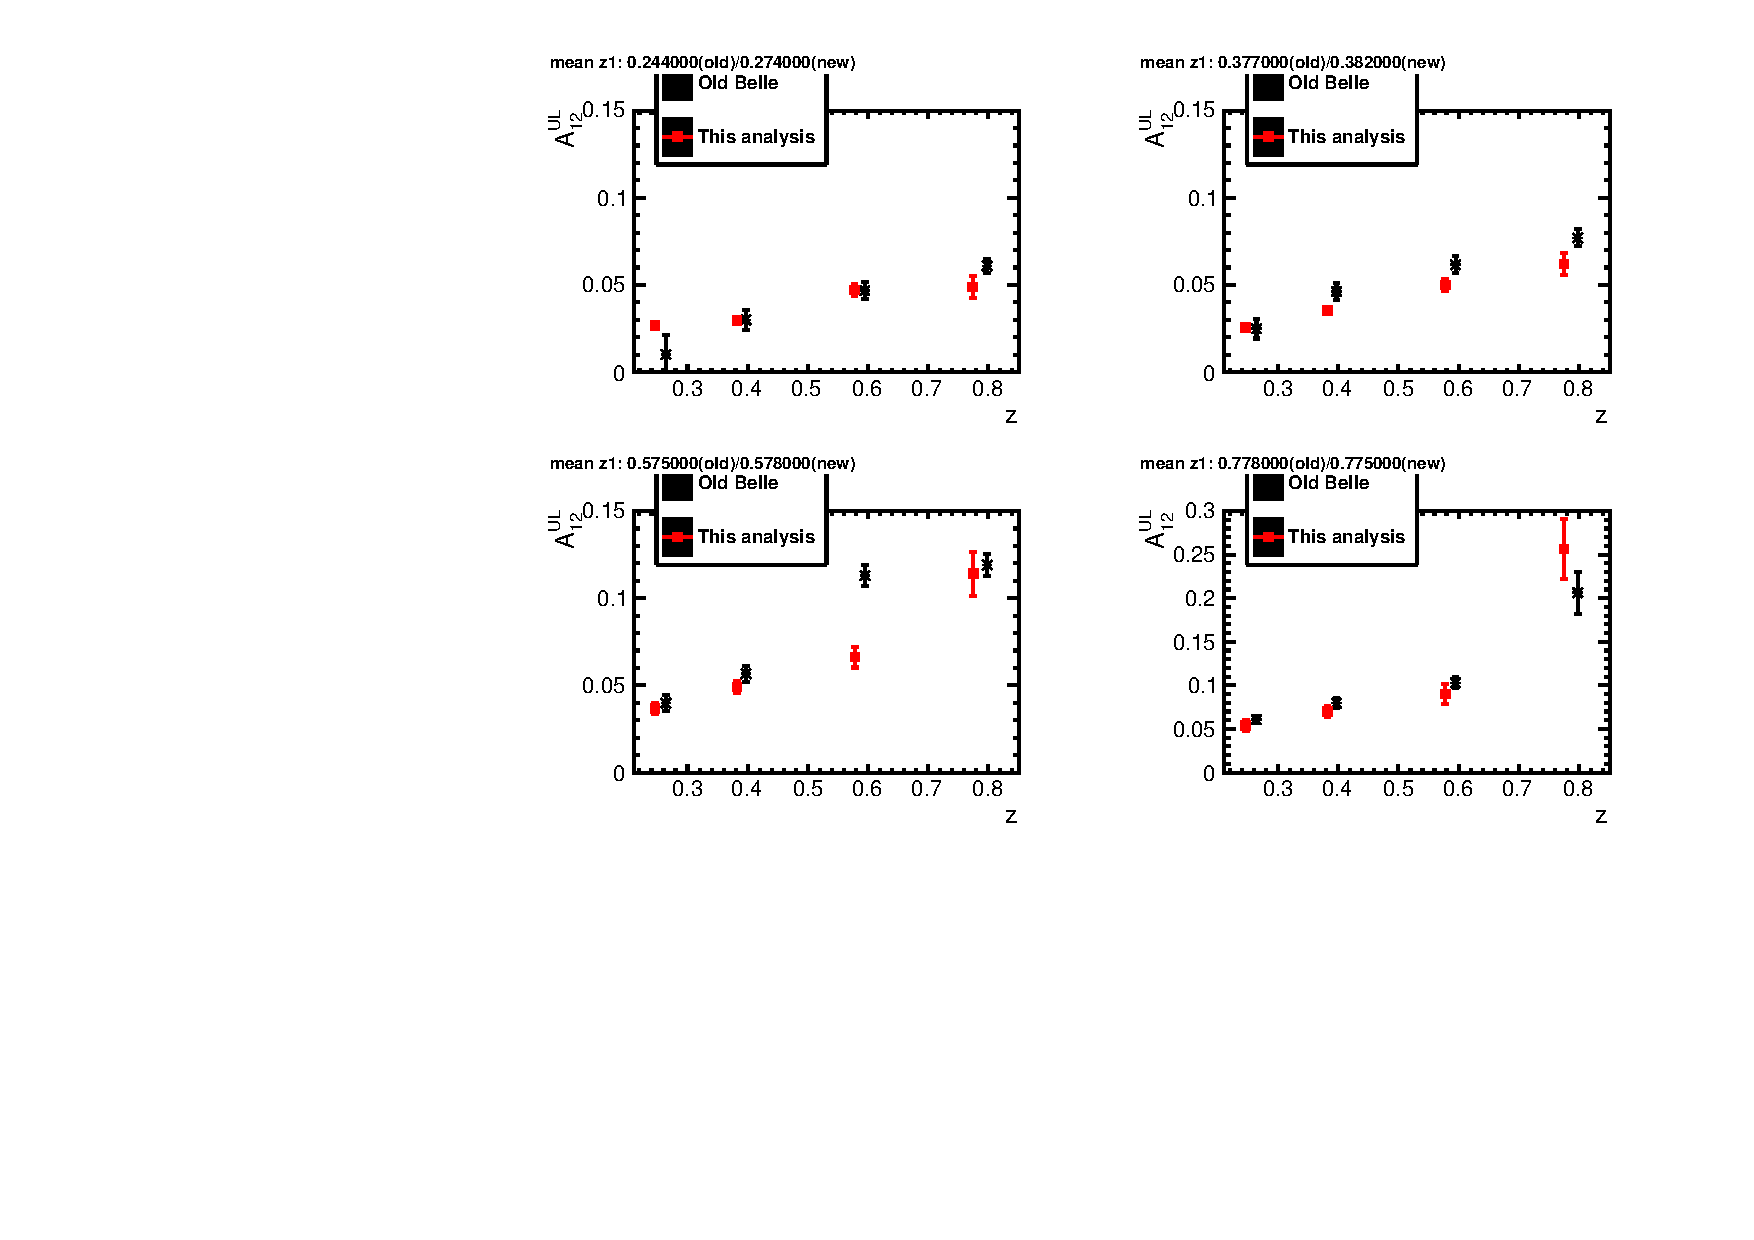
\includegraphics[width=0.95\textwidth]{figure_asy/BelleCompZ25CharmCorr.pdf}
\caption[Comparison of the values for $A^{UL}_{12}$ extracted in this analysis including charm correction and the previous Belle analysis in the ($z_1$, $z_2$) binning]{\label{fig:belleCompCharmCorr} Comparison of the values for $A^{UL}_{12}$ extracted in this analysis and the previous Belle analysis in the ($z_1$, $z_2$) binning. We omitted the lowest $z$ bin since the previous analysis used a cut of $z>0.2$. In addition we applied a charm correction with the assumption that the charm asymmetry is zero. Data points are offset by 0.02 in $z$ for legibility.}
\end{figure}


The results for the non-charm corrected comparison are shown in Fig.~\ref{fig:belleComp}. 
The correction is necessary since the previous Belle results were corrected for the charm contribution.
\begin{figure}[t]
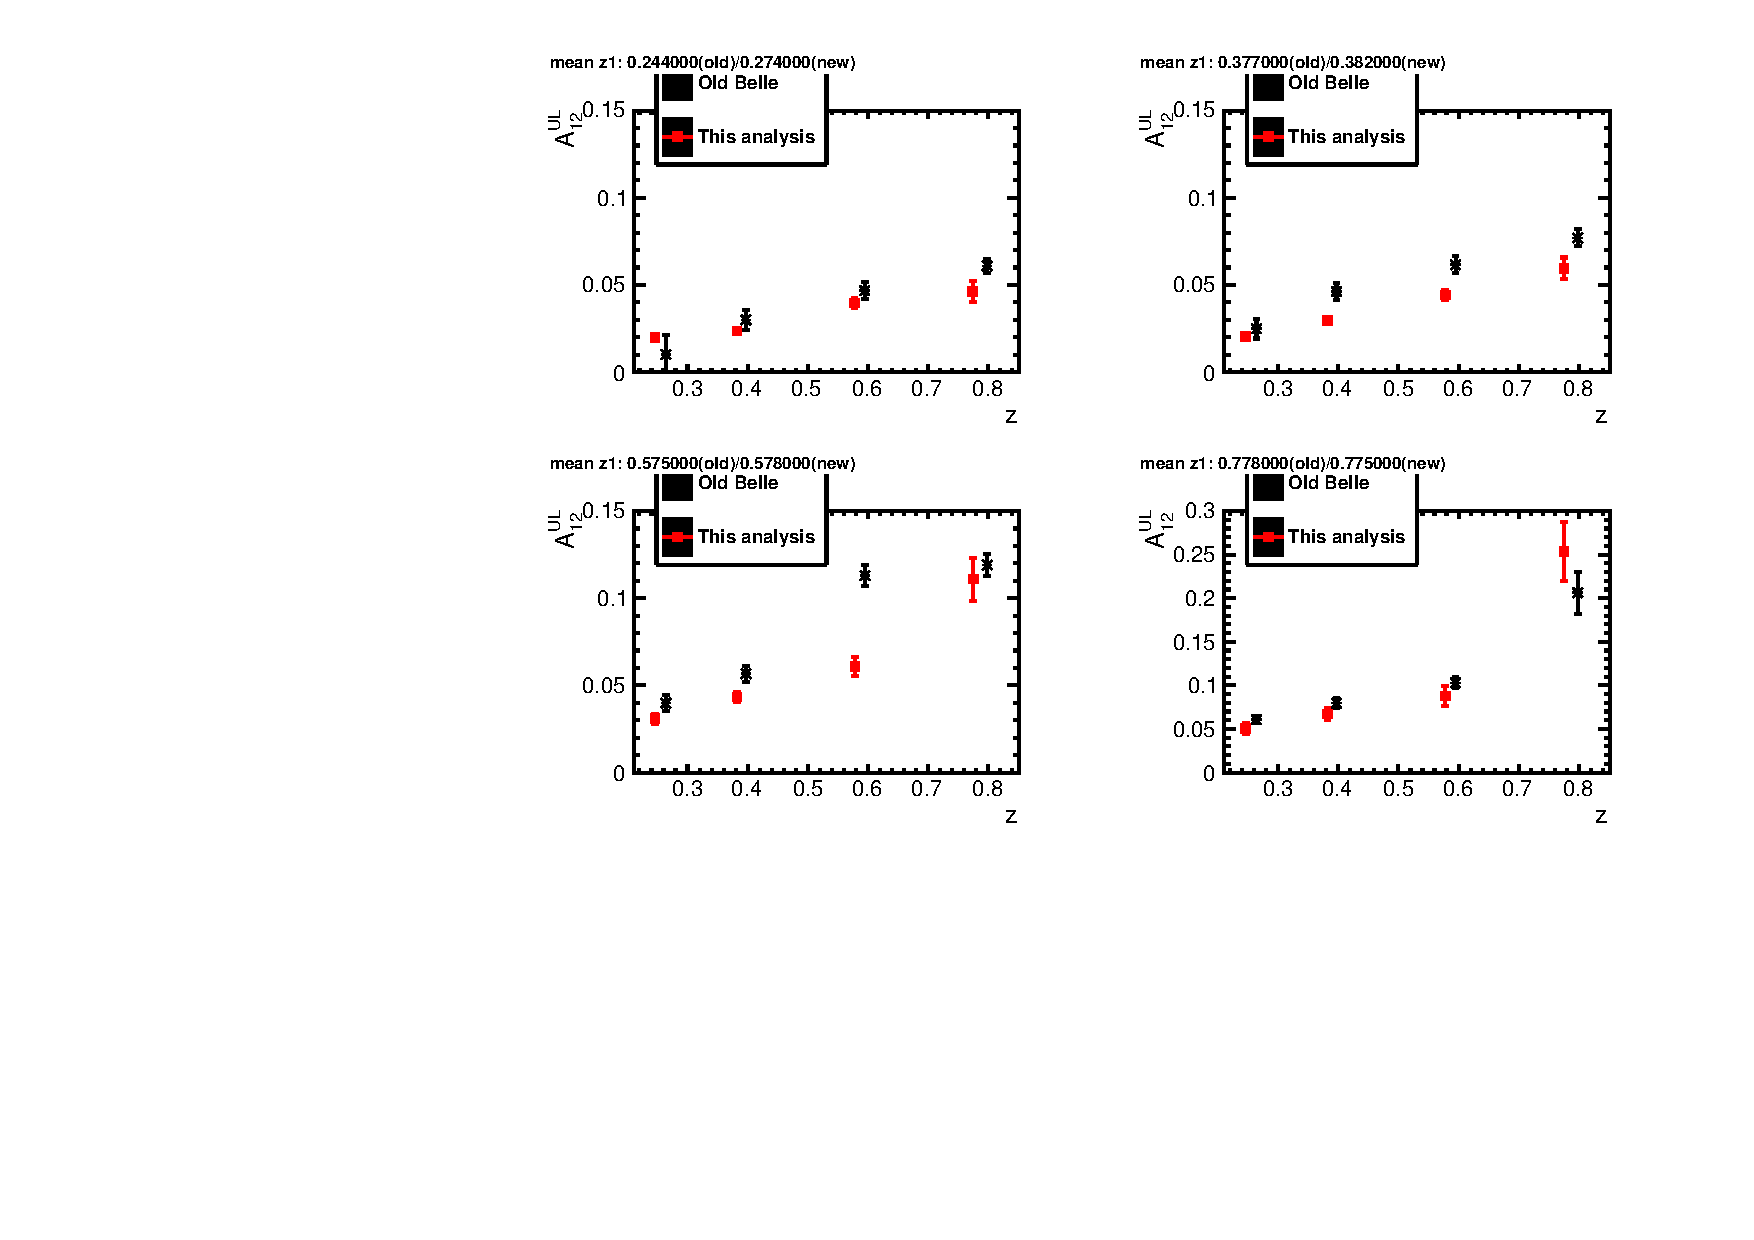
\includegraphics[width=0.95\textwidth]{figure_asy/BelleCompZ25.pdf}
\caption[Comparison of the values for $A^{UL}_{12}$ extracted in this analysis without charm correction and the previous Belle analysis in the ($z_1$, $z_2$) binning]{\label{fig:belleComp} Comparison of the values for $A^{UL}_{12}$ extracted in this analysis and the previous Belle analysis in the ($z_1$, $z_2$) binning without applying a charm correction. We omitted the lowest $z$ bin since the previous analysis used a cut of $z>0.2$. Data points are offset by 0.02 in $z$ for legibility.}
\end{figure}

Figure~\ref{fig:pionCN} displays the comparison of UL, UC, and $\pi^0$ double-ratio asymmetries. The $\pi^0$ double-ratio asymmetry is lower than the UL double ratio, and it is close to the UC ratios. After correcting for the thrust-smearing effect, in Fig.~\ref{fig:pionCNcorrection}, the result for charged pions in the last $(z_1,z_2)$ bin is around 0.25 with large uncertainties. 

\begin{figure}
  \centering     
  \subfigure[$z_1$ bins]{\label{fig:sinzCN1}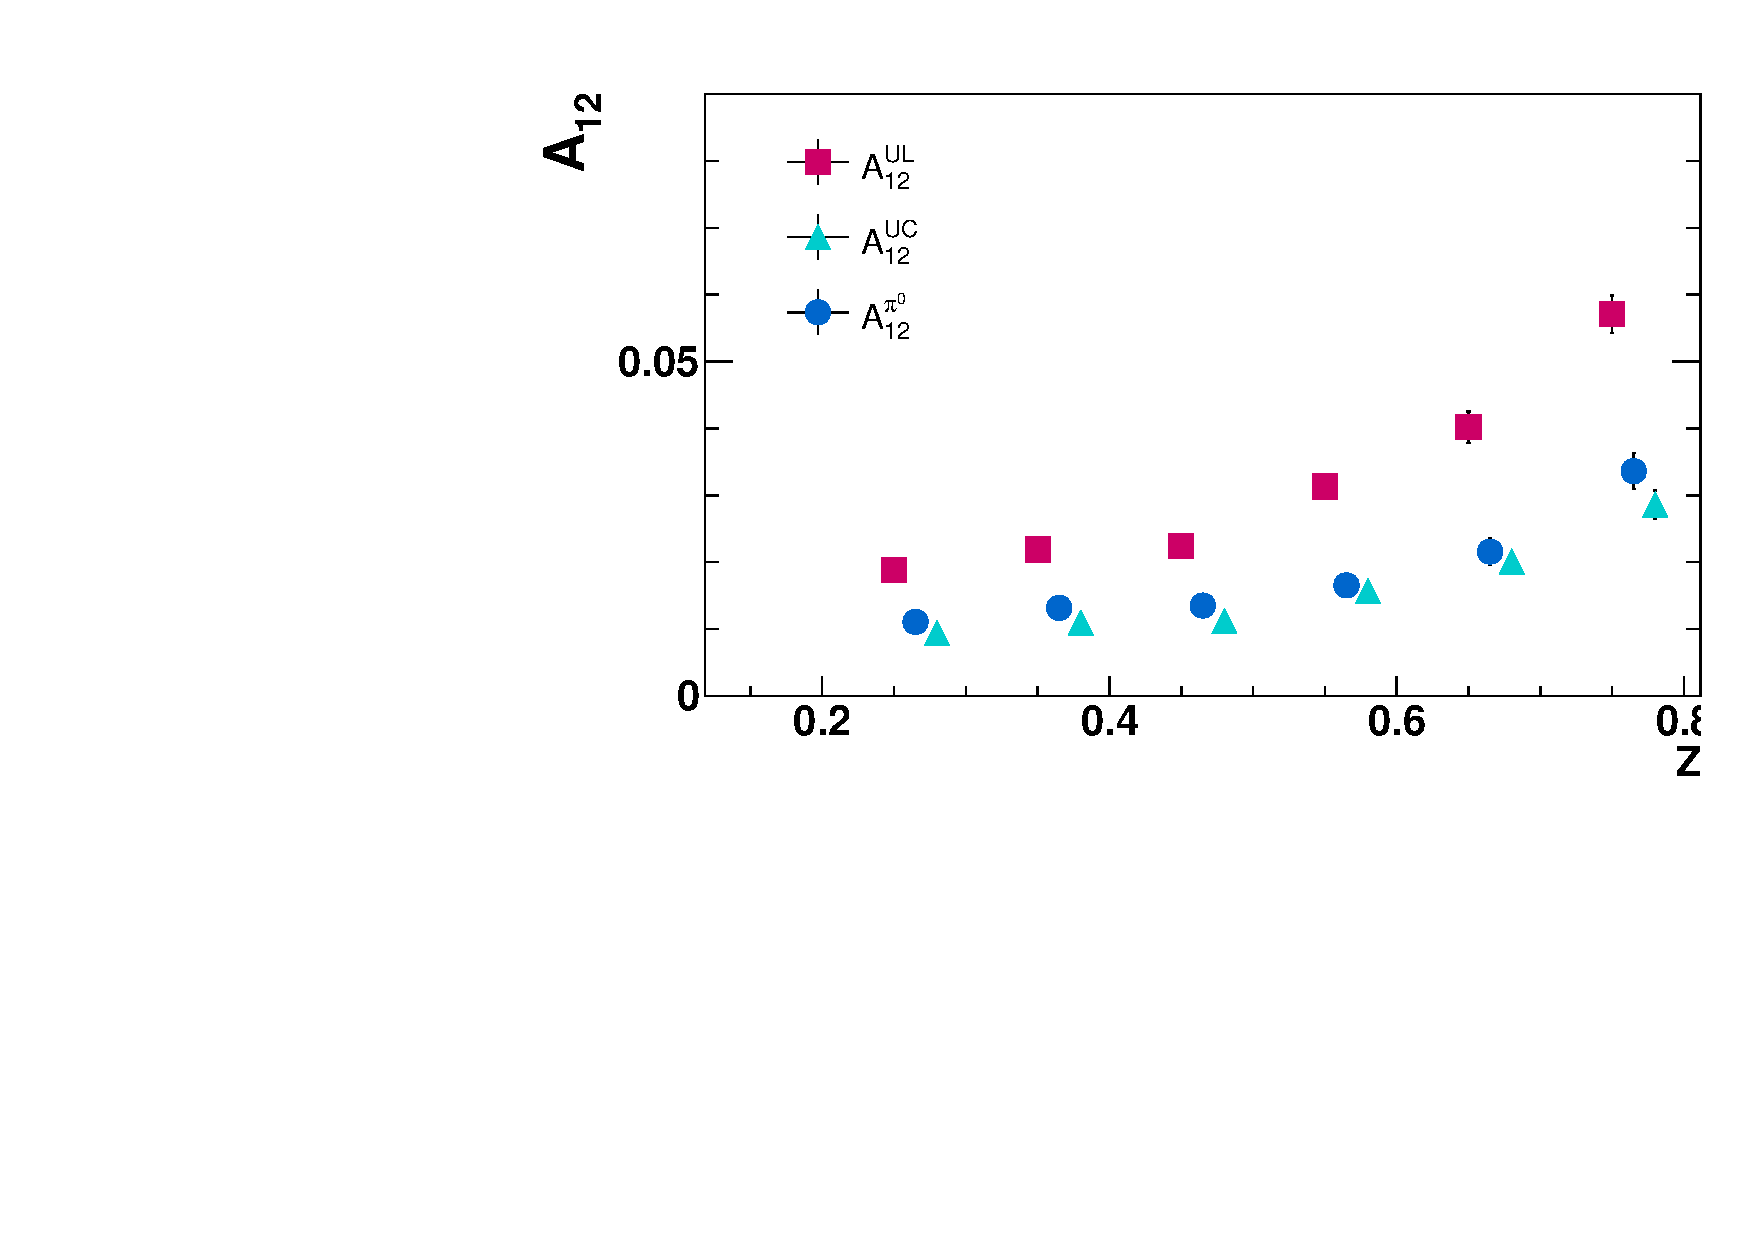
\includegraphics[width=60mm,natwidth=600,natheight=400]{figure_asy/NeutralVsCharge0.pdf}}
  \subfigure[$P_{t1}$ bins]{\label{fig:sinptCN1}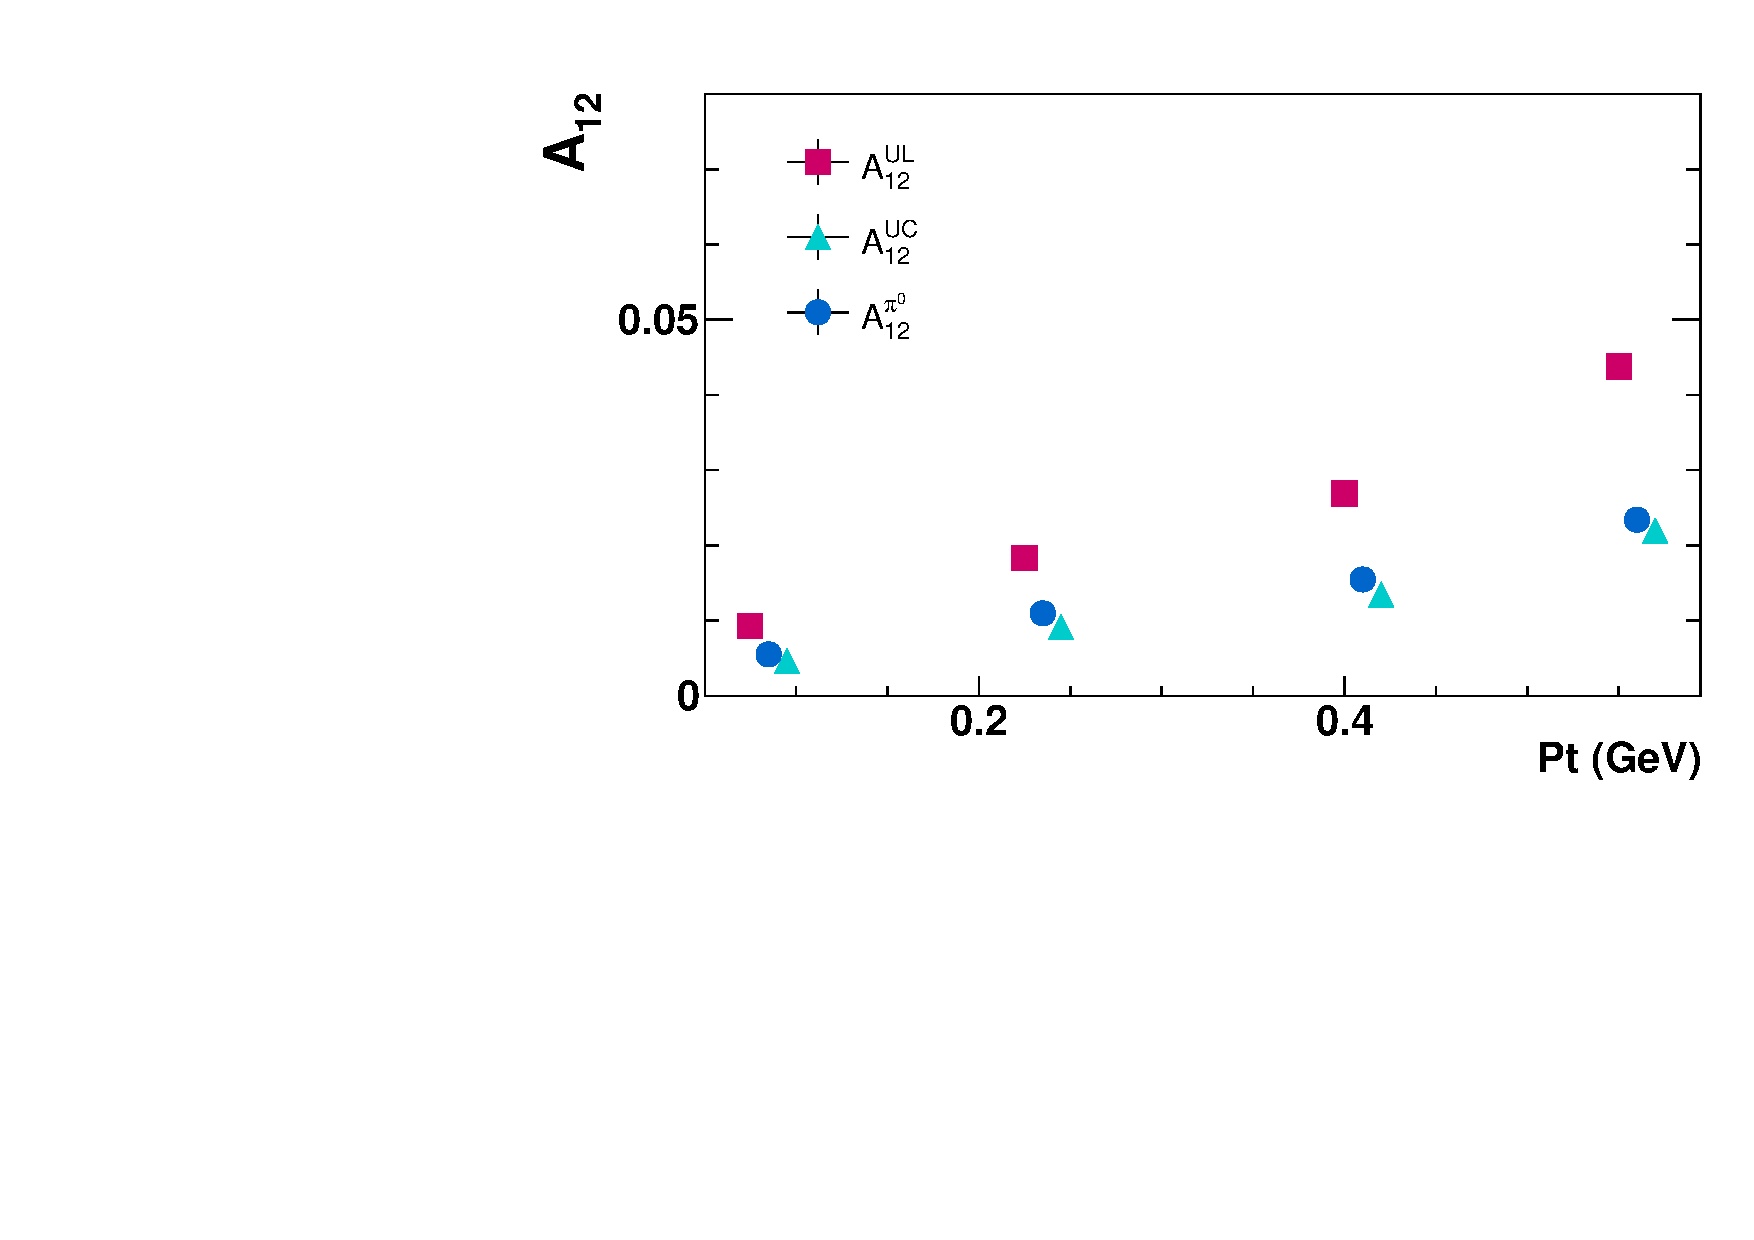
\includegraphics[width=60mm,natwidth=600,natheight=400]{figure_asy/NeutralVsCharge2.pdf}}
  \subfigure[$(z_1,z_2)$ bins]{\label{fig:comzCN1}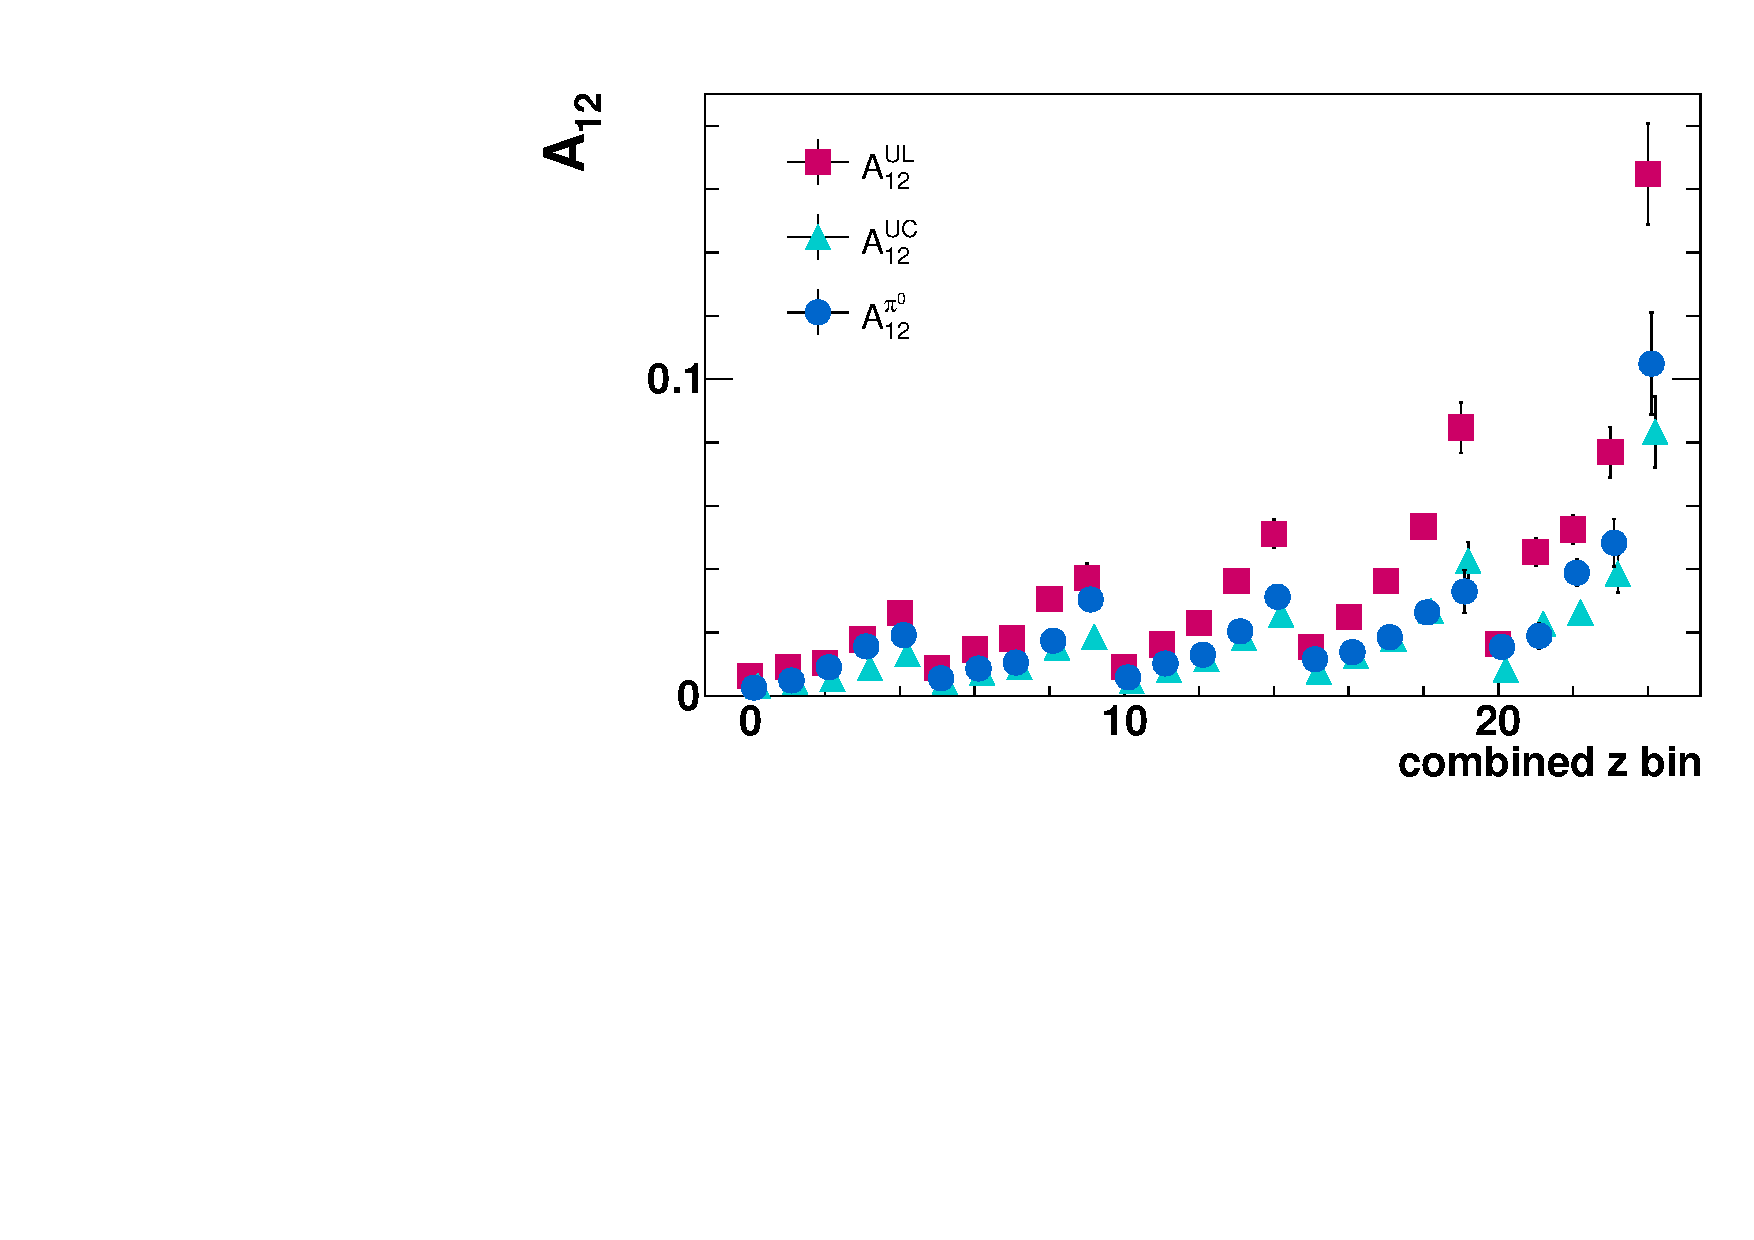
\includegraphics[width=60mm,natwidth=600,natheight=400]{figure_asy/NeutralVsCharge1.pdf}}
  \subfigure[$(P_{t1},P_{t2})$ bins]{\label{fig:comptCN1}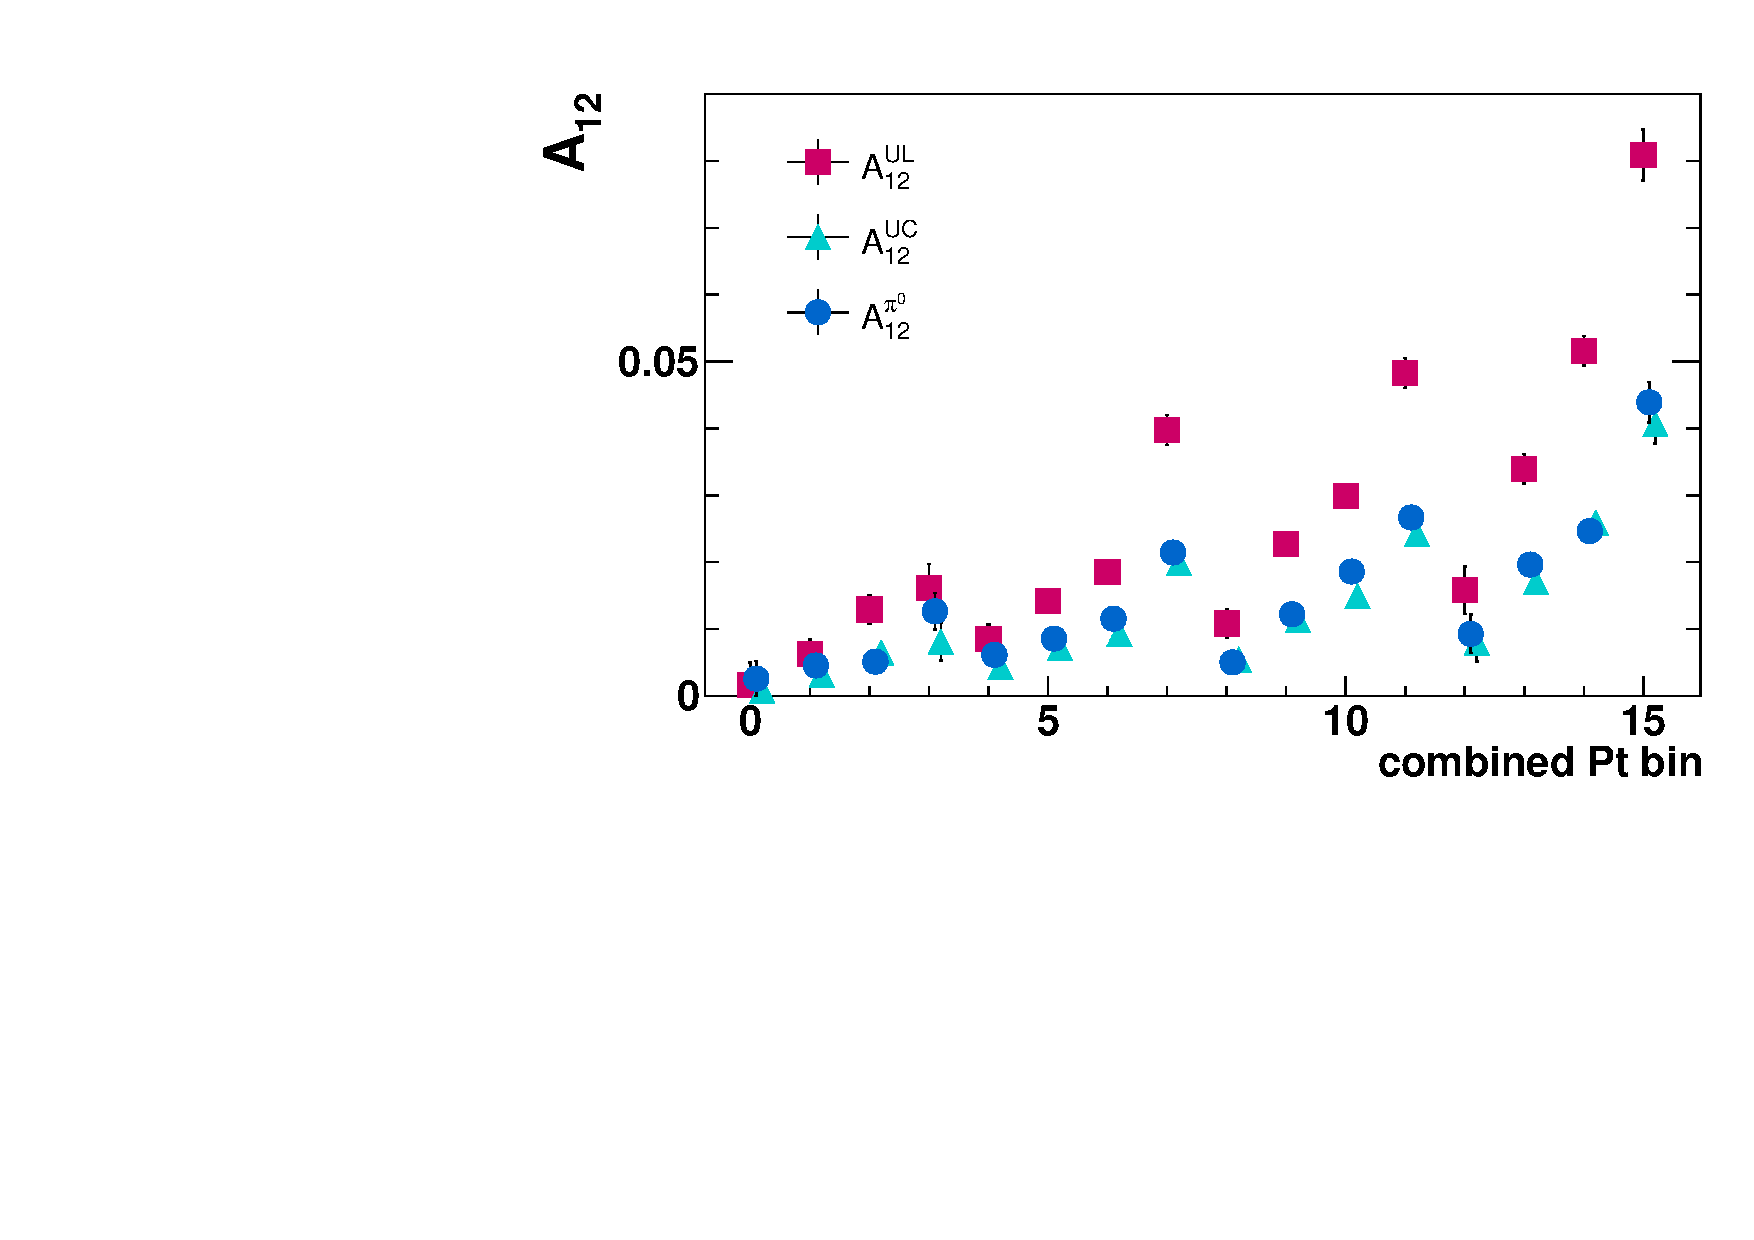
\includegraphics[width=60mm,natwidth=600,natheight=400]{figure_asy/NeutralVsCharge3.pdf}}
  \caption[Charged-pion and $\pi^0$ double ratios before thrust-smearing correction.]{Charged-pion and $\pi^0$ double ratios versus $z$ or $P_t$. The $\pi^0$ double ratios include background correction. The squares, triangles, and points are UL, UC, and $\pi^0$ asymmetries, respectively.}
\label{fig:pionCN}
\end{figure}

\begin{figure}
  \centering     
  \subfigure[$z_1$ bins]{\label{fig:sinzCN2}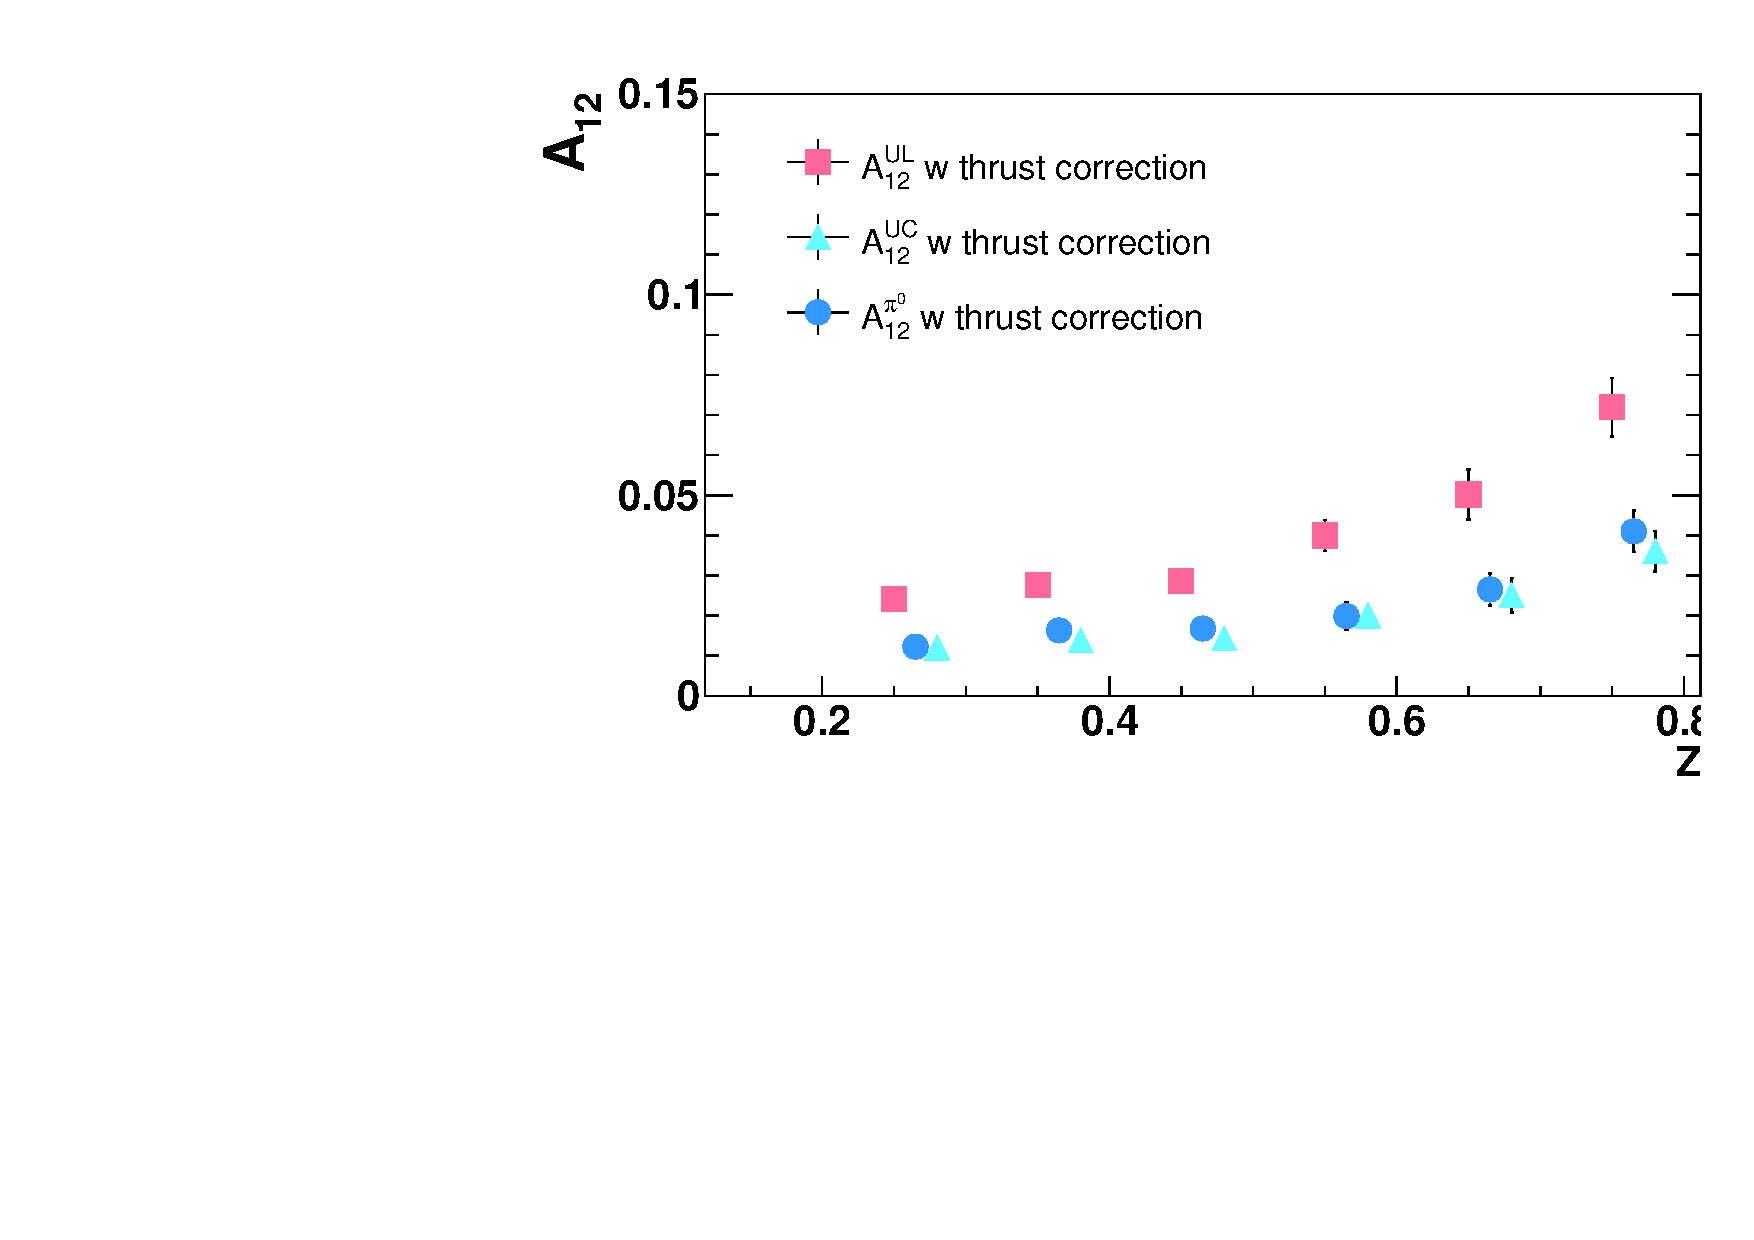
\includegraphics[width=60mm,natwidth=600,natheight=400]{figure_asy/NeutralVsCharge_w_correction0.pdf}}
  \subfigure[$P_{t1}$ bins]{\label{fig:sinptCN2}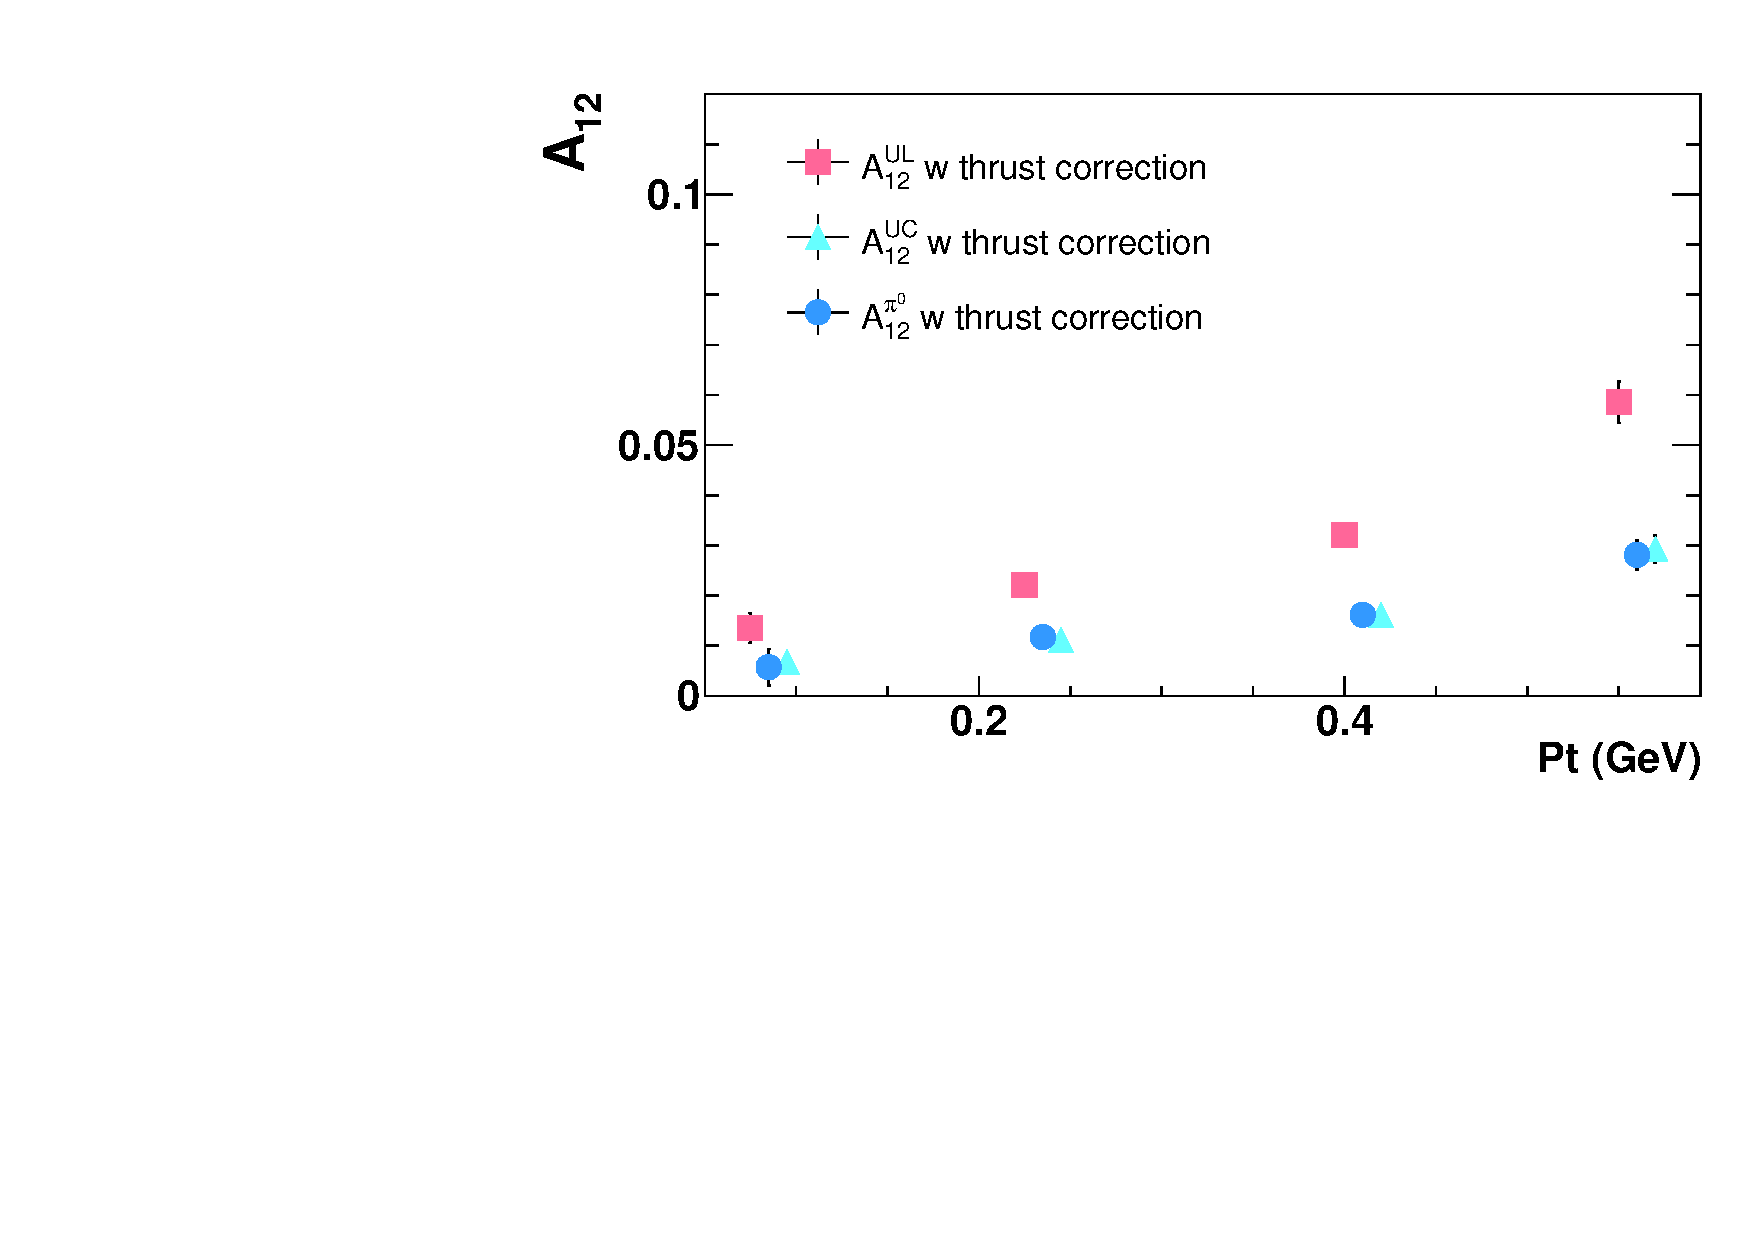
\includegraphics[width=60mm,natwidth=600,natheight=400]{figure_asy/NeutralVsCharge_w_correction2.pdf}}
  \subfigure[$(z_1,z_2)$ bins]{\label{fig:comzCN2}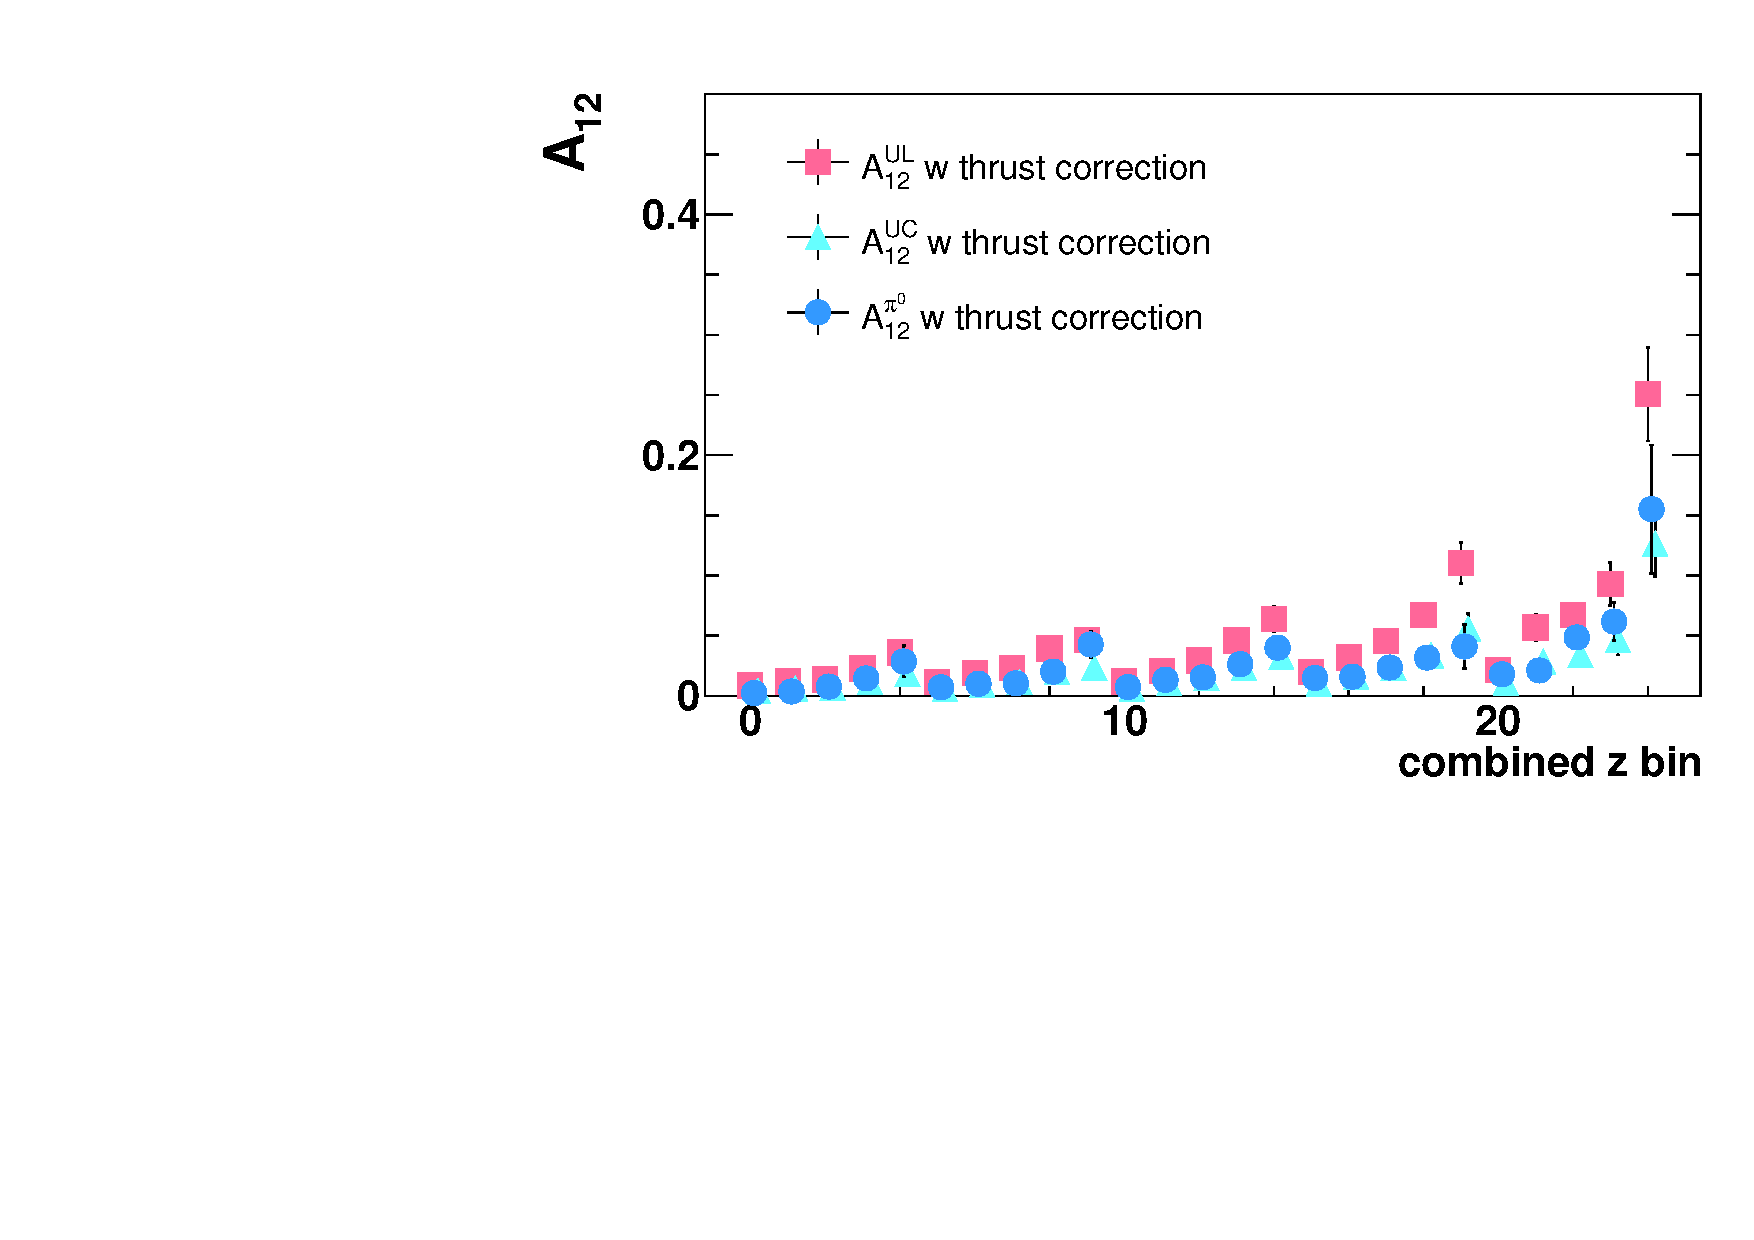
\includegraphics[width=60mm,natwidth=600,natheight=400]{figure_asy/NeutralVsCharge_w_correction1.pdf}} 
  \subfigure[$(P_{t1},P_{t2})$ bins]{\label{fig:comptCN2}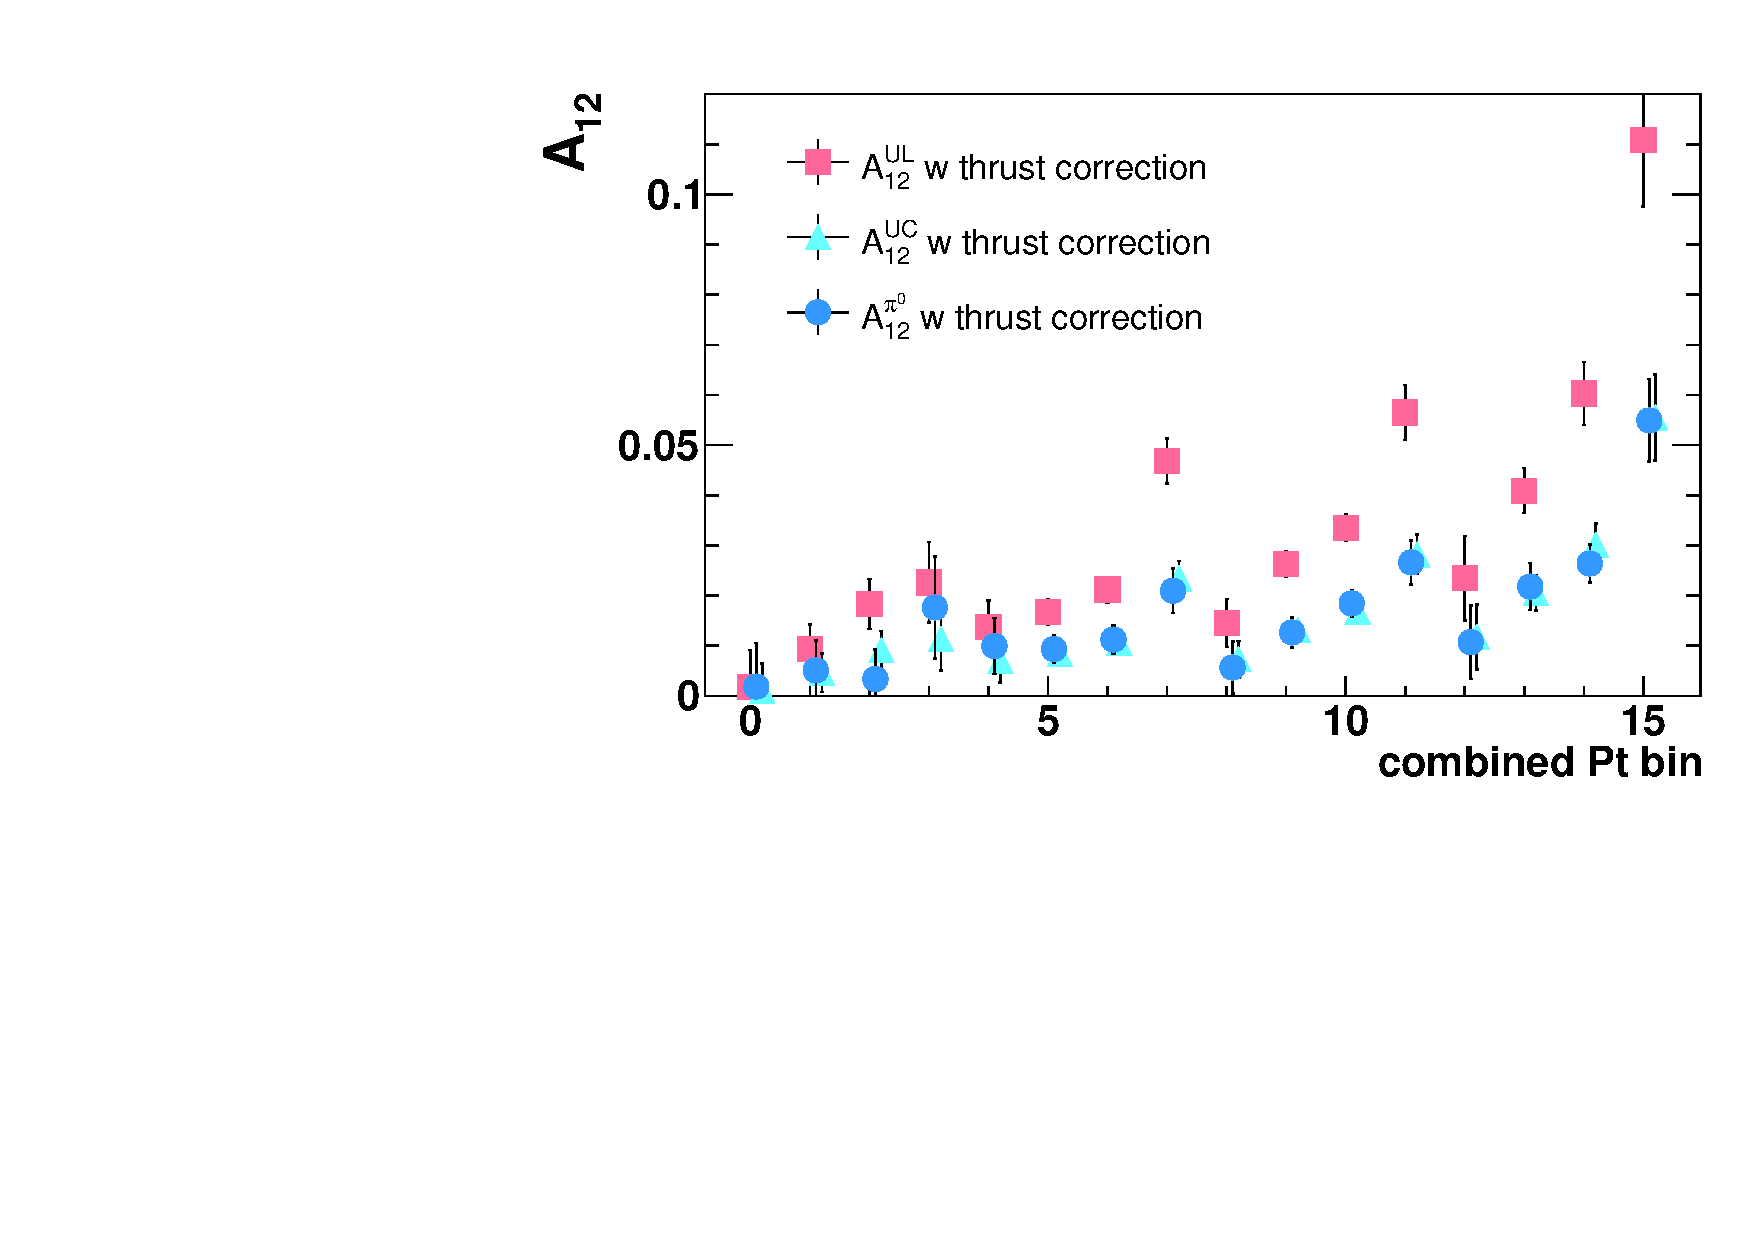
\includegraphics[width=60mm,natwidth=600,natheight=400]{figure_asy/NeutralVsCharge_w_correction3.pdf}}
  \caption[Charged-pion and $\pi^0$ double ratios after thrust-smearing correction.]{Charged-pion and $\pi^0$ double ratios after thrust-smearing correction. The $\pi^0$ double ratios include background correction. The squares, triangles and points are UL, UC, and $\pi^0$ asymmetries, respectively.}
\label{fig:pionCNcorrection}
\end{figure}


%In \cite{BabarCharged}, the Collins asymmetry for charged pions is measured using a data sample collected by the  BaBar collaboration.
%However there are some crucial differences between the work presented in this note and the BaBar results. Most importantly, the BaBar results are corrected with respect to the $q\bar{q}$ axis obtained from leading order MC. They also apply charm and mis-PID corrections. Furthermore, the binning used is different. However, it is worth to note that for the z bin that are the same, our results are consistent and the shape of the asymmetries in $z$, $P_t$ also seem to be consistent.
%studies, mis-PID correction and charm contribution are not considered and the thrust smearing correction factors are applied on the corresponding bins while the other two researches use a average correction factor. Also the smearing correciton factor was calculated using real $q\bar{q}$ axis in previous studies while here we use stable thrust axis. 

%And tighter fiducial constraint applied may increase the statistical uncertainties as well as the Collins asymmetry. Different kinematic bins are assigned and only the bin with $0.5<z_1<0.7, 0.5<z_2<0.7$ is the same with $(z_1,z_2)$ bins 7 in this note. The comparison is listed in Table~\ref{tab:compare}. There are many possible reasons for the difference between measurement. In this note mis-PID correction and charm contribution are not considered and the thrust smearing correction factors are applied on the corresponding bins while the other two researches use a average correction factor. Also tighter fiducial constraint may increase the statistical uncertainties as well as the Collins asymmetry.

\iffalse  
\begin{table}[H]\footnotesize
\centering
\begin{tabular}{|l|l|l|l|l|l|l|l|l|l|l|l|l|l|l|l|l|l|}
\hline
$z_1$ & $z_2$ &  Babar & Belle previous &This Note \\ \hline
UL&[0.5,0.7]&[0.5,0.7]& 10.97$\pm$0.73$\pm$0.62& 11.30$\pm$0.26$\pm$0.53 & 9.97$\pm$0.68-0.13/+0.67 \\ \hline   
UC&[0.5,0.7]&[0.5,0.7]&4.56$\pm$0.6$\pm$0.37&   & 5.37$\pm$0.52-0.13/+0.37 \\ \hline
\end{tabular}
\caption{Variables and results of background correction for $\pi^0$ $z_1$ bins. All numbers are in percent.}
\label{tab:compare}
\end{table}
\fi
